\section{Methodology}
In this section, we first give a definition of the High Uncertainty Area (HUA). Then, we theoretically analyze the existing limitation of ERN in HUA. Based on our analysis, we propose a novel solution to the problem. Finally, we extend our analysis and propose solutions to variants of ERN with other prior distributions.

\subsection{High Uncertainty Area (HUA) of ERN}
In this section, we show that in the high uncertainty area of ERN, the gradient of ERN will shrink to zero, therefore the outputs of ERN cannot be correctly updated. In this paper, we only study the gradient with respect to $\alpha$ as the gradient with respect to $v$ and $\beta$ follows a similar fashion.
\begin{definition}[\textbf{High Uncertainty Area}]
\textit{High Uncertainty Area is where $\alpha$ is close to 1, leading to very high uncertainty prediction.} 
\end{definition}
% We use $\boldsymbol{o}=(o_{\gamma}, o_{v}, o_{\alpha}, o_{\beta})$ to denote the output of $f_{\boldsymbol{\theta}}(X)$, therefore:
% \begin{equation}
% \begin{aligned}
%     \alpha&=\operatorname{SoftPlus}(o_{\alpha}) + 1 \Rightarrow \alpha = \log(\exp(o_{\alpha})+1)+1 \\
%     v&=\operatorname{SoftPlus}(o_v)  \Rightarrow v = \log(\exp(o_v)+1) \\
%     \beta&=\operatorname{SoftPlus}(o_{\beta})  \Rightarrow \beta = \log(\exp(o_{\beta})+1)
% \end{aligned}
% \end{equation}
% Where $\operatorname{SoftPlus}(\cdot)$ denotes $\operatorname{SoftPlus}$ activation. For a sample $X_i$, zero gradient area with respect to $\alpha$ is thus defined where:
% \begin{equation}
%     \frac{\partial \mathcal{L}^{\mathrm{ERN}}}{\partial o_\alpha} = 0
% \end{equation}
% And zero gradient area with respect to $v$ and $\beta$ follows a similar fashion.


% For samples in zero gradient area, the gradient becomes zero, therefore the output cannot be updated. Under such circumstances, the model cannot learn anything from the samples.
An effective model ought to possess the capacity to learn from the entire training samples. Unfortunately, this does not hold true in the context of ERN.
\begin{theorem}
\label{proof1}
\textit{ERN cannot learn from samples in high uncertainty area.}
\end{theorem}

\begin{proof}
Consider input $X$ and the corresponding label $y$. We use $\boldsymbol{o}=(o_{\gamma}, o_{v}, o_{\alpha}, o_{\beta})$ to denote the output of $f_{\boldsymbol{\theta}}(X)$, therefore:
\begin{equation}
\begin{aligned}
\alpha&=\operatorname{SoftPlus}(o_{\alpha}) + 1  \\
      &= \log(\exp(o_{\alpha})+1)+1 
\end{aligned}
\end{equation}
Where $\operatorname{SoftPlus}(\cdot)$ denotes $\operatorname{SoftPlus}$ activation (our theorem still holds true when faced with other popular activation functions, such as $\operatorname{ReLU}$ and $\operatorname{exp}$, see Appendix~\ref{appendix_1} for additional proofs). 
So the gradient of NLL loss with respect to $o_{\alpha}$ is given by:
\begin{equation}
\begin{aligned}
\frac{\partial \mathcal{L}^{\mathrm{NLL}}}{\partial o_\alpha} &= \frac{\partial \mathcal{L}^{\mathrm{NLL}}}{\partial \alpha} \frac{\partial \alpha}{\partial o_{\alpha}}     \\
&=[\log(1+\frac{\nu(\gamma-y)^2}{2\beta(\nu+1)}) +\psi(\alpha) \\
&- \psi(\alpha+0.5)] \cdot \operatorname{Sigmoid}\left(o_\alpha\right)
\end{aligned}
\end{equation}
where $\psi(\cdot)$ denotes the digamma function.

For a sample in high uncertainty area, we have:
\begin{equation}
    \alpha \rightarrow 1 \Rightarrow o_\alpha \rightarrow-\infty \Rightarrow \operatorname{Sigmoid}\left(o_\alpha\right) \rightarrow 0
\end{equation}
So, for such training samples:
\begin{equation}
    \frac{\partial \mathcal{L}^{\mathrm{NLL}}}{\partial o_\alpha} = 0
\end{equation}

And the gradient of $\mathcal{L}^{\mathrm{R}}=|y-\gamma| \cdot(2 v+\alpha)$ with respect to $o_{\alpha}$ is given by:
\begin{equation}
\begin{aligned}
    \frac{\partial \mathcal{L}^{\mathrm{R}}}{\partial o_\alpha}&=\frac{\partial \mathcal{L}^{\mathrm{R}}}{\partial \alpha} \frac{\partial \alpha}{\partial o_\alpha} \\
    &= |y-\gamma| \cdot \operatorname{Sigmoid}\left(o_\alpha\right)
\end{aligned}
\end{equation}
Similarly, we have:
\begin{equation}
    \frac{\partial \mathcal{L}^{\mathrm{R}}}{\partial o_\alpha} = 0
\end{equation}
And $\mathcal{L}^{\mathrm{ERN}}=\mathcal{L}^{\mathrm{NLL}}+\lambda \mathcal{L}^{\mathrm{R}}$, therefore we have:
\begin{equation}
\begin{aligned}
\frac{\partial \mathcal{L}^{\mathrm{ERN}}}{\partial o_\alpha} &= \frac{\partial \mathcal{L}^{\mathrm{NLL}}}{\partial o_\alpha} +\lambda \frac{\partial \mathcal{L}^{\mathrm{R}}}{\partial o_\alpha} \\
&=0
\end{aligned}
\end{equation}
\end{proof}

Since the gradient of the loss function with respect to $o_{\alpha}$ is zero, there won't be any update on $\alpha$ from such samples. The model fails to learn from samples in high uncertainty area.

\subsection{Uncertainty Regularization To Bypass HUA}
Considering the learning deficiency of ERN, in this paper, we propose an uncertainty regularization to solve the zero gradient problem within HUA:
\begin{equation}
    \mathcal{L}^{\mathrm{U}} =  -| y-\gamma | \cdot  \log(\exp(\alpha-1)-1) 
\end{equation}
% where $\lambda_{U}$ is a settable hyperparameter.
In this section, we show that $\mathcal{L}^{\mathrm{U}}$ can address the learning deficiency of ERN.
\begin{theorem}
\textit{Our proposed uncertainty regularization $\mathcal{L}^{\mathrm{U}}$ can learn from samples within HUA.}
\end{theorem}

\begin{proof}
The gradient of proposed regularization term $\mathcal{L}^{\mathrm{U}}$ with respect to $o_{\alpha}$ is given by:
\begin{equation}
\begin{aligned}
\frac{\partial \mathcal{L}^{\mathrm{U}}}{\partial o_\alpha} &= \frac{\partial \mathcal{L}^{\mathrm{U}}}{\partial \alpha} \frac{\partial \alpha}{\partial o_{\alpha}}     \\
&=-| y-\gamma | \cdot \frac{\exp (\alpha-1)}{\exp (\alpha-1)-1} \cdot \operatorname{Sigmoid}\left(o_\alpha\right) \\
&=-| y-\gamma | \cdot \left[1+\exp \left(-o_\alpha\right)\right] \cdot \frac{1}{1+\exp \left(-o_\alpha\right)} \\
&=-| y-\gamma |
\end{aligned}
\end{equation}
\end{proof}
Uncertainty regularization term $\mathcal{L}^{\mathrm{U}}$ ensures the maintenance of the gradient within the high uncertainty area. Importantly, the value of this gradient scales in accordance with the distance between the predicted value and the ground truth.

\begin{figure}
\centering
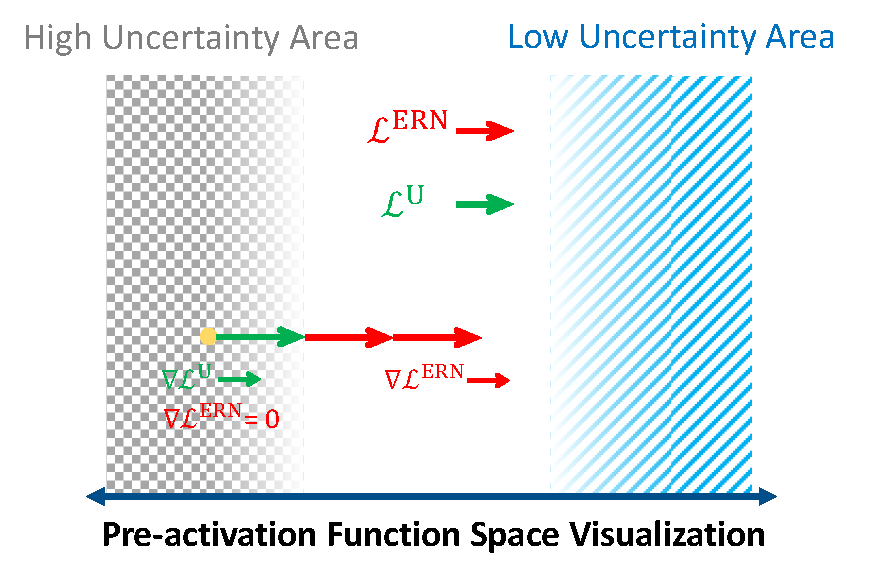
\includegraphics[width=0.9\columnwidth]{Uncertainty} % Reduce the figure size so that it is slightly narrower than the column. Don't use precise values for figure width.This setup will avoid overfull boxes.
\caption{$\mathcal{L}^{\mathrm{ERN}}$ in Equation~\eqref{eq:ern-loss} cannot help the model get out of high uncertainty area while our proposed $\mathcal{L}^{\mathrm{U}}$ can still learn from samples in the grey area.}
\label{uncertainty_visualization}
\end{figure}


\subsubsection{Training of Regularized ERN}
The final training objective for the proposed Uncertainty Regularized ERN (UR-ERN) is formulated as:
\begin{equation}
    \mathcal{L} = \mathcal{L}^{\mathrm{ERN}} +\lambda_{1} \mathcal{L}^{\mathrm{U}}
\end{equation}
where $\lambda_{1}$ is a settable hyperparameter that balances the regularization and the original ERN loss. $\mathcal{L}^{\mathrm{NLL}}$ is for fitting purpose, $\mathcal{L}^{\mathrm{R}}$ regularizes evidence~\cite{NEURIPS2020_aab08546}. And our proposed $\mathcal{L}^{\mathrm{U}}$ addresses zero gradient problem in the HUA. %high uncertainty area.

\subsubsection{Uncertainty Space Visualization}
Figure~\ref{uncertainty_visualization} visualizes the uncertainty space with $x$-axis representing $o_{\alpha}$. Under ideal conditions, both fitting loss and uncertainty should be low, resulting in samples being mapped to the blue zone. Nevertheless, there exist certain samples predicted with high uncertainty, which may land within the grey region. Within this grey region, $\mathcal{L}^{\mathrm{ERN}}$ fails to update the parameters effectively. Under such circumstances, our proposed uncertainty regularization term $\mathcal{L}^{\mathrm{U}}$ retains the capacity to update the model. This enables the samples to be extracted from the grey area, thus allowing the training to continue.


\subsection{Uncertainty Regularization for ERN Variants}
Based on our theoretical analysis in previous sections, it is quite clear that the zero gradient problem in the HUA of ERN is attributable to certain activation functions that ensure non-negative values. Consequently, this limitation is not confined to ERN but can also extend to other evidential models that utilize similar activation functions. Multivariate ERN~\cite{meinert2021multivariate}, which we introduced in Section~\ref{sec:back:variant}, serves as an illustrative example; it suffers from similar problems to ERN, even when employing different prior distributions. Similar to the previous analysis, we study the parameter $\nu$ as an example. 

\begin{theorem}
\textit{Multivariate ERN~\cite{meinert2021multivariate} also cannot learn from samples in high uncertainty area.}
\end{theorem}

\begin{proof}
Given the output of a NN $\left(p_1 \cdots p_m\right)$, we have $p_\nu \in\left(p_1 \cdots p_m\right)$. And $\nu$ is formulated as the following:
\begin{equation}
    \nu = n(n+5)/2+\tanh p_{\nu} \cdot  n(n+3)/2  + 1
\end{equation}
Therefore, the gradient of loss function $\mathcal{L}^{\mathrm{MERN}}$ ($\mathcal{L}^{\mathrm{NLL}}$) with respect to $p_{\nu}$ is given by:
\begin{equation}
\begin{aligned}
\frac{\partial \mathcal{L}^{\mathrm{MERN}}}{\partial p_{\nu}}&=\frac{\partial \mathcal{L}^{\mathrm{NLL}}}{\partial \nu} \frac{\partial \nu}{\partial p_{\nu}} \\
&=\frac{\partial \mathcal{L}^{\mathrm{NLL}}}{\partial \nu} \cdot \frac{n(n+3)}{2} \cdot (1-\tanh^2 p_{\nu})
\end{aligned}
\end{equation}
within HUA, we have:
\begin{equation}
        p_{\nu} \rightarrow -\infty \Rightarrow (1-\tanh^2 p_{\nu}) \rightarrow 0 
\end{equation}
Therefore, we have:
\begin{equation}
    \frac{\partial \mathcal{L}^{\mathrm{MERN}}}{\partial p_{\nu}} = 0
\end{equation}

The gradient with respect to $p_{\nu}$ is zero, there will be no update to $p_{\nu}$. Multivariate ERN cannot learn effectively within HUA.
\end{proof}

Similarly, we propose uncertainty regularization term $\mathcal{L}^{\mathrm{U}}$ to help Multivariate ERN learn from samples within HUA. Since Multivariate ERN uses a different activation function, the proposed $\mathcal{L}^{\mathrm{U}}$ for Multivariate ERN has a different formulation:
\begin{equation}
    \mathcal{L}^{\mathrm{U}} = -\frac{1}{2} \cdot|y-\gamma| \cdot \log(\frac{n^2 + 3n}{n^2 + 4n+1-\nu}-1)
\end{equation}
We can prove the effectiveness of the proposed $\mathcal{L}^{\mathrm{U}}$ for Multivariate ERN. 


\begin{theorem}
\textit{Our proposed uncertainty regularization $\mathcal{L}^{\mathrm{U}}$ can help Multivariate ERN learn from samples within HUA.}
\end{theorem}

\begin{proof}
The gradient of the proposed $\mathcal{L}^{\mathrm{U}}$ with respect to $p_{\nu}$ is given by:
\begin{equation}
\begin{aligned}
\frac{\partial \mathcal{L}^{\mathrm{U}}}{\partial p_{\nu}} &= \frac{\partial \mathcal{L}^{\mathrm{U}}}{\partial \nu} \frac{\partial \nu}{\partial p_{\nu}}     \\
&=-| y-\gamma | \cdot \frac{1}{2(n^2+3n)} \\
&\cdot \frac{-(n^2 + 3n)^2}{(\nu-n-1)(\nu-n^2-4n-1)} \\
&\cdot \frac{n^2+3n}{2} \cdot (1-\tanh^2 p_{\nu}) \\
&=-| y-\gamma | \cdot  \frac{1}{2(n^2+3n)} \\
&\cdot \frac{-(n^2 + 3n)^2}{(\nu-n-1)(\nu-n^2-4n-1)}\\
&\cdot \frac{n^2+3n}{2} \cdot \frac{-4(\nu-n-1)(\nu-n^2-4n-1)}{(n^2 + 3n)^2} \\
&=-| y-\gamma | 
\end{aligned}
\end{equation}

\end{proof}

The proposed regularization term $\mathcal{L}^{\mathrm{U}}$ guarantees a non-zero gradient for Multivariate ERN in the HUA. Therefore, the loss function for uncertainty regularized Multivariate ERN is formulated as:
\begin{equation}
    \mathcal{L}=\mathcal{L}^{\mathrm{NLL}}+\lambda_1 \mathcal{L}^{\mathrm{U}}
\end{equation}
where $\lambda_1$ is settable hyperparameter.

While the two terms have different formulations, they share a common intuition. We identify the zero gradient problem arising from the activation function and introduce a term to circumvent zero gradients, simultaneously increasing $\alpha$.
%avoid zero gradients and increase $\alpha$.
This adjustment guides the training process away from this problematic area.
%guiding training away from this problematic area. 
Our mathematical analysis confirms these terms effectively achieve our objective.

The above theoretical analysis reveals that the learning deficiency is not exclusive to ERN~\cite{NEURIPS2020_aab08546}; it also manifests in other evidential models~\cite{meinert2021multivariate} that employ different prior distributions. 


% The above theoretical analysis reveals that the learning deficiency is not exclusive to ERN~\cite{NEURIPS2020_aab08546}; it also manifests in other evidential models~\cite{meinert2021multivariate} that employ different prior distributions. Importantly, our proposed method offers a universal solution, enabling these models to overcome this challenge.

% \begin{figure}
% \centering
% 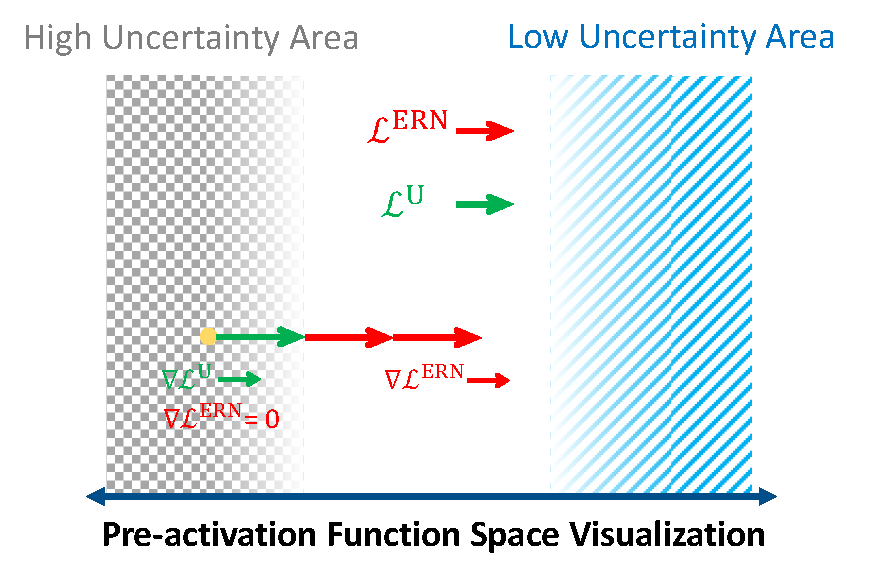
\includegraphics[width=0.9\columnwidth]{Uncertainty} % Reduce the figure size so that it is slightly narrower than the column. Don't use precise values for figure width.This setup will avoid overfull boxes.
% \caption{$\mathcal{L}^{\mathrm{ERN}} = \mathcal{L}^{\mathrm{NLL}}+\lambda_1 \mathcal{L}^{\mathrm{R}}$ cannot help the model get out of high uncertainty area while our proposed $\mathcal{L}^{\mathrm{U}}$ can still learn from samples in the grey area.}
% \label{uncertainty_visualization}
% \end{figure}


% \begin{figure}
%     \centering
%     \begin{subfigure}{0.33\columnwidth}
%         \centering
%         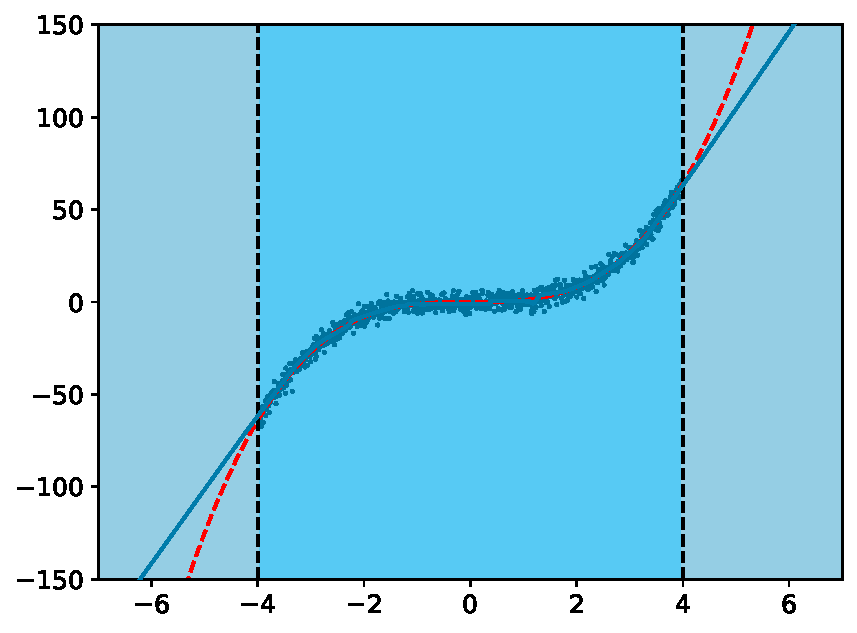
\includegraphics[width=0.95\linewidth]{toy_ERN.pdf}
%         \caption{ERN}
%         \label{fig:sub11}
%     \end{subfigure}%
%         \begin{subfigure}{0.33\columnwidth}
%         \centering
%         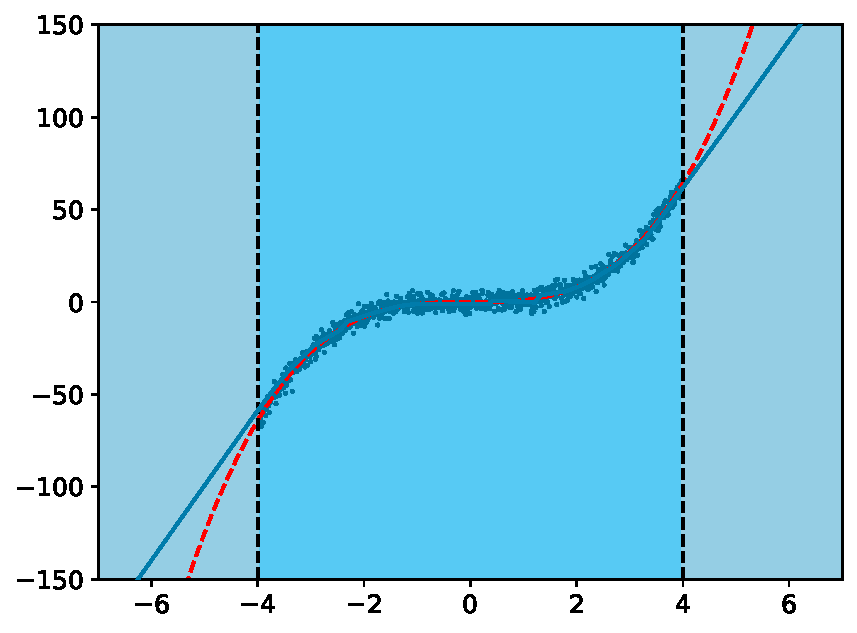
\includegraphics[width=0.95\linewidth]{toy_NLL.pdf}
%         \caption{NLL-ERN}
%         \label{fig:sub12}
%     \end{subfigure}
%     \begin{subfigure}{0.33\columnwidth}
%         \centering
%         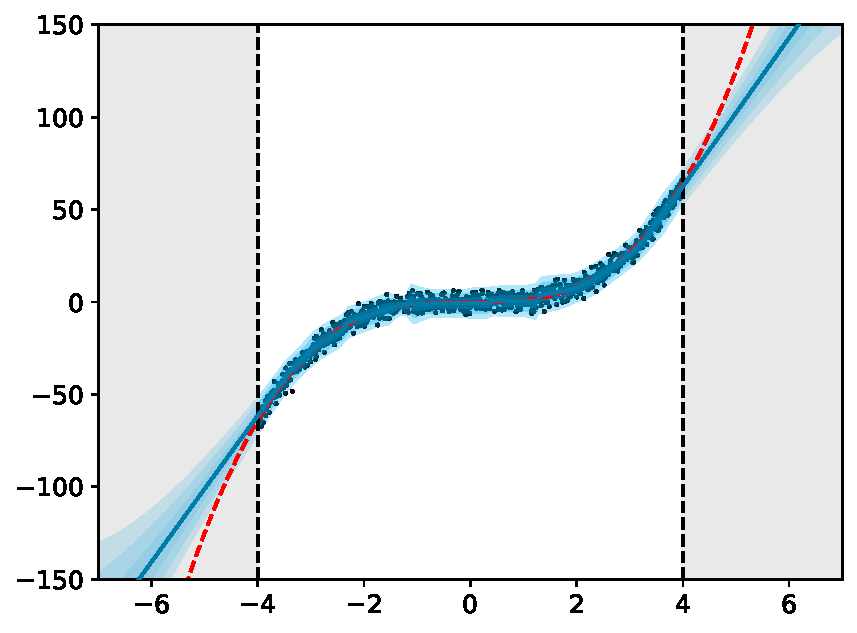
\includegraphics[width=0.95\linewidth]{toy_URERN.pdf}
%         \caption{UR-ERN}
%         \label{fig:sub13}
%     \end{subfigure}
%     \caption{ERN, NLL-ERN, and UR-ERN performance comparison on Cubic Regression Dataset. The training and testing regions are segmented by two dotted lines. The dataset's training samples are depicted as black points. Ground truth values are represented by a red dotted curve. The predictive mean is traced by a blue curve, while the surrounding blue shading indicates the extent of predictive uncertainty.}
%     \label{fig:toy_dataset}
% \end{figure}
